\chapter{L'introduction}
Un terminal est un périphérique de \textit{I/O} \footnote {L'entrée/sortie (Input/Output en anglais, abrégé E/S) permet à l'utilisateur d'envoyer des données (par exemple, à l'aide du clavier) et de recevoir des données en sortie (par exemple, via l'écran)} qui permet d'intéragir avec un système d'exploitation. Au tout début, un terminal était physique (comme le \textit{VT-100}) doté d'un clavier et d'un écran. Comme le périphérique ne disposait pas de \textit{cerveau}, pour effectuer des calculs informatiques, il devait être impérativement raccordé à un \textbf{mainframe} \footnote{Un ordinateur centrale qui permet d'effectuer des calculs informatiques et possède un réseaux de terminaux qui pouvait être connecter dessus} via le port série RS-232.
\newline
\begin{figure}[h]
	\centering
	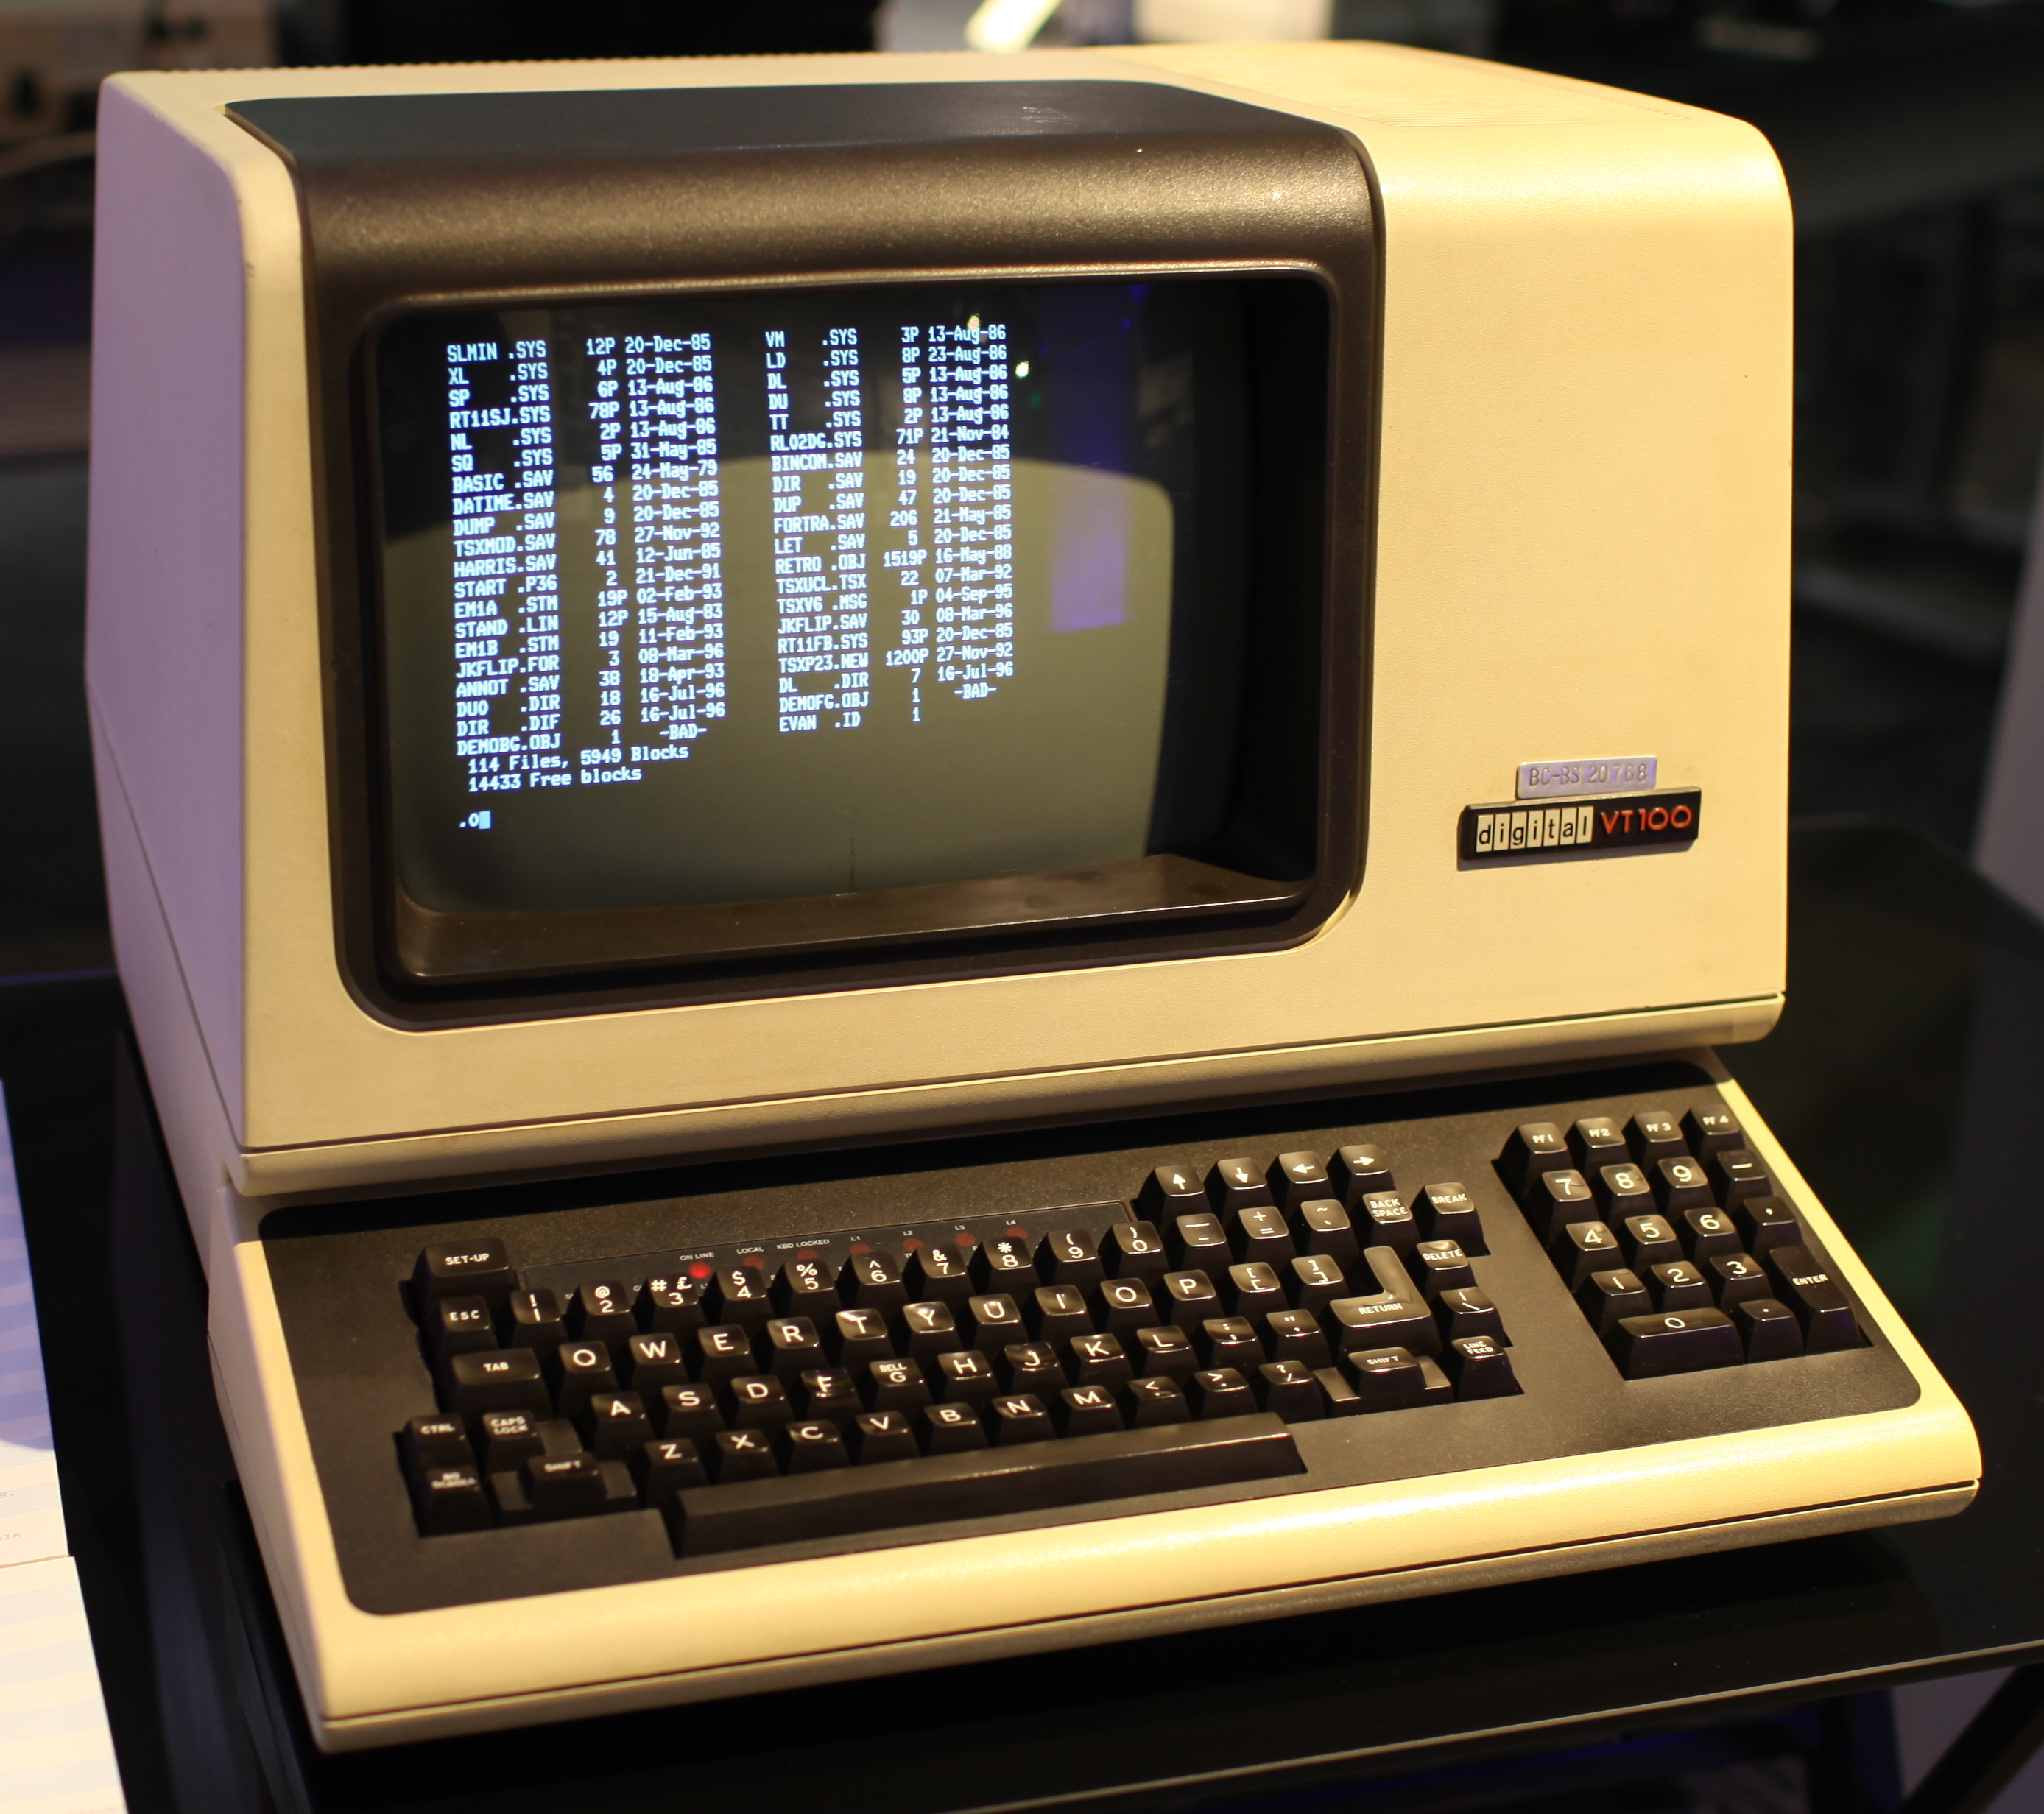
\includegraphics[width=150px, height=150px]{DEC_VT100_terminal.jpg}
	\caption{Un terminal physique VT-100}
\end{figure}
\newline
Les commandes entrées dans le clavier du terminal physique étaient envoyées vers le mainframe à travers le câble RS-232, et le mainframe renvoyait les résultats à son tour qui devaient être affichés sur l'écran. Mais après l'apparition des ordinateurs personnels, le terminal physique n'était plus nécessaire, car il était capable d'effectuer les mêmes tâches que le mainframe, c'est-à-dire effectuer des calculs informatiques, entre autres.
